\documentclass[journal]{IEEEtran}
\usepackage{cite}
\usepackage{amsmath,amssymb}
\usepackage{graphicx}
\usepackage{booktabs}
\usepackage{multirow}
\usepackage{url}
\usepackage{tikz}
\usetikzlibrary{arrows.meta,positioning,calc}
\usepackage{circuitikz}
\ctikzset{bipoles/length=0.9cm}
\graphicspath{{figures/}}
% auto-generated by sim/make_figures.py -- do not edit
\providecommand{\nfzeroMHz}{1,001}
\providecommand{\nQi}{22,393}
\providecommand{\nQc}{179,680}
\providecommand{\nQL}{17,925}
\providecommand{\nQe}{16,640}
\providecommand{\nILmeas}{28.20}
\providecommand{\nTdrop}{13.98}
\providecommand{\nILidt}{14.22}
\providecommand{\nRm}{2,261}
\providecommand{\nLmH}{6.44}
\providecommand{\nCmaF}{3.92}
\providecommand{\nCzeropF}{0.85}
\providecommand{\nRzerok}{20.00}
\providecommand{\nRs}{4.00}
\providecommand{\nkeff}{4.61}
\providecommand{\nFSRMHz}{5.72}
\providecommand{\nradiusum}{100.15}
\providecommand{\ntaurtns}{174.80}
\providecommand{\nart}{0.98}
\providecommand{\ntcp}{1.00}
\providecommand{\nkappatwo}{0.61}
\providecommand{\nGazeromS}{5.53}
\providecommand{\nNidt}{20}
\providecommand{\nLin}{29.80}
\providecommand{\nLt}{60.00}
\providecommand{\nQLind}{8.00}
\providecommand{\nIone}{3.00}
\providecommand{\nItwo}{3.00}
\providecommand{\nIfour}{2.00}
\providecommand{\nLttwo}{40.00}
\providecommand{\nRptanktwo}{2,013}
\providecommand{\nPdc}{28.80}
\providecommand{\nIdc}{16.00}
\providecommand{\nvdd}{1.80}
\providecommand{\ngmone}{30.00}
\providecommand{\ngmtwo}{30.00}
\providecommand{\ngmfour}{20.00}
\providecommand{\nZTideal}{151,968}
\providecommand{\nZTeff}{33,828}
\providecommand{\nTzeroideal}{34.90}
\providecommand{\nTzero}{21.85}
\providecommand{\nkimpl}{-13.05}
\providecommand{\ntrim}{12.80}
\providecommand{\nRext}{174.67}
\providecommand{\nFmodel}{6.38}
\providecommand{\nFused}{6.64}
\providecommand{\nPs}{-2.47}
\providecommand{\nVportone}{1.66}
\providecommand{\nRptank}{3,019}
\providecommand{\ntaug}{5.70}
\providecommand{\nZin}{66.67}
\providecommand{\nmaz}{175}
\providecommand{\nFpartRm}{0.00}
\providecommand{\nFpartresother}{-13.21}
\providecommand{\nFpartLin}{-2.14}
\providecommand{\nFpartdriver}{-23.03}
\providecommand{\nFpartCG}{3.52}
\providecommand{\nFparttank}{-3.77}
\providecommand{\nFpartstagetwo}{-19.14}
\providecommand{\nloopLoss}{1.65}
\providecommand{\nloopLossNoL}{2.34}
\providecommand{\ngmcrit}{64.64}
\providecommand{\ngmthreex}{193.93}
\providecommand{\nPthreex}{27.93}
\providecommand{\nwindow}{2,310}
\providecommand{\ntauStart}{0.47}
\providecommand{\ntStart}{5.19}
\providecommand{\nILbestQeight}{14.03}
\providecommand{\nILbestQthreezero}{8.49}
\providecommand{\nILrecQeight}{14.17}
\providecommand{\nmodeMargin}{1.70}
\providecommand{\nmodeCompK}{2}
\providecommand{\nmodeCompMHz}{11.44}
\providecommand{\nNopt}{87.50}
\providecommand{\nmarginNopt}{40.00}
\providecommand{\nmarginBase}{1.70}
\providecommand{\nngTzero}{21.85}
\providecommand{\nngPhase}{0.00}
\providecommand{\nngFosc}{1,000}
\providecommand{\nngDf}{-177.07}
\providecommand{\nngWarp}{-692.71}
\providecommand{\nngHstep}{14.50}
\providecommand{\nngFoscCorr}{1,001}
\providecommand{\nngVpone}{1.66}
\providecommand{\nngIm}{0.71}
\providecommand{\nngPrm}{-2.47}
\providecommand{\nngTstart}{3.35}
\providecommand{\nngHDtwo}{-8.25}
\providecommand{\nngHDthree}{-9.68}
\providecommand{\nngTHD}{71.69}
\providecommand{\nngF}{6.64}
\providecommand{\nngCt}{195.65}
\providecommand{\nngCttwo}{498.81}
\providecommand{\nngLin}{31.29}
\providecommand{\nPNonekfconezerok}{-127.74}
\providecommand{\nPNonezerokfconezerok}{-154.70}
\providecommand{\nPNonezerozerokfconezerok}{-166.94}
\providecommand{\nPNoneMfconezerok}{-167.68}
\providecommand{\nPNonekfcthreezerok}{-123.24}
\providecommand{\nPNonezerokfcthreezerok}{-151.69}
\providecommand{\nPNonezerozerokfcthreezerok}{-166.21}
\providecommand{\nPNoneMfcthreezerok}{-167.60}
\providecommand{\nPNonekfconezerozerok}{-118.11}
\providecommand{\nPNonezerokfconezerozerok}{-147.29}
\providecommand{\nPNonezerozerokfconezerozerok}{-164.34}
\providecommand{\nPNoneMfconezerozerok}{-167.31}
\providecommand{\nPNonek}{-123.24}
\providecommand{\nPNonezerok}{-151.69}
\providecommand{\nPNonezerozerok}{-166.21}
\providecommand{\nPNoneM}{-167.60}
\providecommand{\nPNfloor}{-167.73}
\providecommand{\nhalfBW}{30.08}
\providecommand{\nFoMonezerozerok}{231.63}
\providecommand{\nFoMonek}{228.66}
\providecommand{\nFoMoneM}{213.01}
\providecommand{\nPNonezerozerokQthreezero}{-157.79}
\providecommand{\nFQthreezero}{7.23}
\providecommand{\nPNonezerozerokQfive}{-158.91}
\providecommand{\nmcN}{300}
\providecommand{\nmcTzeromean}{21.69}
\providecommand{\nmcTzerostd}{3.56}
\providecommand{\nmcTzeromin}{9.71}
\providecommand{\nmcYield}{100.00}
\providecommand{\nmcPNonezerozeromean}{-158.57}
\providecommand{\nmcPNonezerozerostd}{1.69}
\providecommand{\nmcPNonemean}{-115.42}
\providecommand{\nmcPNonestd}{2.12}
\providecommand{\nmcQeMean}{16,475}
\providecommand{\nmcQeStd}{2,874}
\providecommand{\nmcTrimMin}{-3.21}
\providecommand{\nmcTrimMax}{27.34}
\providecommand{\ntempDfRange}{8,750}
\providecommand{\ntempTzeromin}{21.20}
\providecommand{\ntempTzeromax}{22.74}
\providecommand{\ntempPNmin}{-160.31}
\providecommand{\ntempPNmax}{-157.45}
\providecommand{\nadevonems}{3.61\times10^{-11}}
\providecommand{\nadevones}{5.48\times10^{-12}}
\providecommand{\nadevonezerous}{5.10\times10^{-10}}

% fallbacks when the transistor-level or Cadence runs are not available yet
\providecommand{\nngTzero}{n/a}\providecommand{\nngFosc}{n/a}\providecommand{\nngDf}{n/a}\providecommand{\nngVpone}{n/a}
\providecommand{\nngIm}{n/a}\providecommand{\nngPrm}{n/a}\providecommand{\nngTstart}{n/a}\providecommand{\nngHDtwo}{n/a}
\providecommand{\nngHDthree}{n/a}\providecommand{\nngTHD}{n/a}\providecommand{\nngF}{n/a}\providecommand{\nngCt}{n/a}\providecommand{\nngPhase}{n/a}
\newcommand{\dBc}{dBc/Hz}
\newcommand{\tbd}{\textit{post-layout}}

\begin{document}
\title{CMOS Co-Design of a 1-GHz Oscillator on a Low-Loss SiN--LiNbO$_3$ Phononic Ring Resonator: Extended mBVD--Delay Modeling, Impedance-Recovering Sustaining Amplifier and Electronic Mode Selection}

\author{M.~Nisha~Angeline,~\IEEEmembership{Senior Member,~IEEE}
\thanks{M. Nisha Angeline is with the Department of Electronics and Communication Engineering, Velalar College of Engineering and Technology, Thindal, Erode 638012, Tamil Nadu, India (e-mail: nishavlsidesign@gmail.com).}
\thanks{Manuscript prepared October 2026 for submission to the IEEE Transactions on Circuits and Systems I: Regular Papers.}}

\markboth{IEEE Transactions on Circuits and Systems I: Regular Papers}{Nisha Angeline: CMOS Co-Design of a Phononic Ring-Resonator Oscillator}

\maketitle

\begin{abstract}
Phononic integrated circuits on silicon nitride-on-lithium niobate (SiN--LN) have recently delivered gigahertz acoustic ring resonators with loaded quality factors near $\nQL$ and intrinsic $f\!\cdot\!Q$ products above $2\times10^{13}$~Hz, but every oscillator demonstrated so far closes the loop with bench instruments through 50-$\Omega$ interfaces. This paper presents the first complete CMOS co-design for this resonator class. A compact model is derived that augments the modified Butterworth--Van Dyke (mBVD) circuit with a recirculating delay element equal to the ring round-trip time, so that the full mode comb, the group delay and the start-up dynamics of the ring are captured in a Verilog-A cell usable in Spectre PSS/Pnoise. The model is calibrated to the measured $\nfzeroMHz$-MHz device ($Q_L=\nQL$, $Q_i=\nQi$, $Q_c=\nQc$, 28.2-dB insertion loss) and shows that only $\nTdrop$~dB of the measured loss is intrinsic to the ring; the remaining $\nILidt$~dB is transduction and 50-$\Omega$ mismatch that an integrated interface can recover. Because the effective coupling of the two-port ring is $k_{\mathrm{eff}}^2\approx\nkeff\times10^{-6}$, the Pierce topology has an inductive window of $\nwindow$~Hz and is unusable; a transmission-mode differential sustaining amplifier in 180-nm CMOS is designed instead, with C$_0$-resonating centre-tapped port inductors, a common-gate cascode transimpedance input, an LC-tank phase trim and an IDT-pair-count rule ($N\approx f_0/2\,\mathrm{FSR}$) that raises the mode-selection margin from $\nmarginBase$ to $\nmarginNopt$~dB. Transistor-level simulation gives $\nngTzero$~dB of loop gain, a loop noise factor of $\nngF$~dB, start-up in $\nngTstart$~$\mu$s and $\nngPrm$~dBm dissipated in the ring at $\nPdc$~mW. The predicted phase noise is $\nPNonek$, $\nPNonezerok$ and $\nPNonezerozerok$~\dBc\ at 1, 10 and 100~kHz offset (figure of merit $\nFoMonezerozerok$~dB), which places the oscillator between multiplied quartz and the best FBAR references and 25~dB better than FBAR--CMOS oscillators at 100~kHz. Monte Carlo analysis over resonator, inductor and process variations gives a start-up yield of $\nmcYield$\,\% and a 1-$\sigma$ phase-noise spread of $\nmcPNonezerozerostd$~dB. The Cadence Virtuoso/Spectre, layout, DRC/LVS and extraction flow is provided for the post-layout verification.
\end{abstract}

\begin{IEEEkeywords}
Phononic integrated circuits, lithium niobate, ring resonator, sustaining amplifier, phase noise, Verilog-A, Butterworth--Van Dyke model, mode selection, CMOS oscillator.
\end{IEEEkeywords}

\section{Introduction}
\IEEEPARstart{A}{coustic} resonators are the backbone of frequency references because the acoustic wavelength is five orders of magnitude shorter than the electromagnetic one at the same frequency, which gives compact, high-$Q$ devices. Quartz, film bulk acoustic resonators (FBARs) and silicon MEMS resonators are, however, one-port devices whose electromechanical coupling $k_t^2$ sets both the inductive window exploited by Pierce and Colpitts topologies and the tuning range \cite{vittoz1988,hashimoto2009}. Phononic integrated circuits (PnICs) change this picture: guided acoustic waves on lithium niobate (LN) can be routed, split, coupled and stored in waveguide ring resonators in the same way as light in photonic circuits \cite{fu2019,shao2019,mayor2021}. The recently reported silicon nitride-on-lithium niobate (SiN--LN) platform \cite{ji2026} patterns a low-loss SiN waveguide layer on an unpatterned LN substrate and reaches single-mode propagation loss of 1.9~dB/cm, a ring resonator with $Q_L=\nQL$ at $\nfzeroMHz$~MHz ($Q_i=\nQi$, $Q_c=\nQc$, under-coupled) and, with a bench amplifier and phase shifter, an oscillator with $-159$~\dBc\ at 100~kHz offset that tunes from 1000 to 1007~MHz by phase control.

Three obstacles separate that demonstration from an integrated reference oscillator. First, the ring is a two-port transmission device whose measured 28.2-dB insertion loss (IL) in a 50-$\Omega$ system mixes the intrinsic drop-port transfer of the ring with transducer bidirectionality, taper loss and impedance mismatch. Second, the ratio of motional to static capacitance seen between the two interdigital transducers (IDTs) is of order $10^{-6}$, far below the $10^{-2}$ of an FBAR, so the oscillator literature built on parallel-resonance topologies does not apply. Third, the ring supports a comb of azimuthal modes separated by the free spectral range (FSR) with nearly identical loss, so mode selection must be designed, not assumed. None of these issues is visible in a single-branch Butterworth--Van Dyke (BVD) model.

This paper addresses the three obstacles with a complete co-design that goes from the measured resonator to a layout-ready CMOS sustaining amplifier. The contributions are:
\begin{enumerate}
\item an \emph{extended mBVD + delay} compact model of the two-port phononic ring (Section~\ref{sec:model}) whose motional elements are derived from the physical ring quantities ($Q_i$, $Q_c$, FSR, $f_0$) rather than fitted, and whose recirculating delay element reproduces the mode comb and the group delay; the Verilog-A implementation is a floating four-terminal element compatible with Spectre PSS/Pnoise;
\item a quantitative decomposition of the measured IL into a ring-intrinsic part ($\nTdrop$~dB) and a recoverable interface part ($\nILidt$~dB), and the proof that a Pierce oscillator is infeasible for this resonator class (Section~\ref{sec:codesign});
\item a transmission-mode differential sustaining amplifier in 180-nm CMOS with C$_0$-resonating centre-tapped port inductors, a common-gate cascode transimpedance front end with LC-tank phase trim and a loss budget of $\nloopLoss$~dB instead of 28~dB (Section~\ref{sec:amp});
\item an electronic mode-selection scheme based on the half-round-trip phase alternation of the comb and an IDT-pair-count rule, $N\approx f_0/(2\,\mathrm{FSR})$, that places the IDT nulls on the in-phase competitor modes (Section~\ref{sec:mode});
\item transistor-level verification (open-loop gain, noise factor, start-up, steady state), a circuit-derived Leeson--Hajimiri phase-noise budget, Monte Carlo and temperature studies, and a comparison with FBAR, SAW and quartz references (Section~\ref{sec:results}); and
\item a reproducible Cadence Virtuoso flow (Spectre netlists, OCEAN scripts for stb/PSS/Pnoise/corners/Monte Carlo, Calibre DRC/LVS/PEX run scripts) for the post-layout step (Section~\ref{sec:flow}).
\end{enumerate}
All numerical results in this paper are produced by an open-source pipeline (Python and ngspice \cite{ngspice}) released with the manuscript; every number in the text is generated by that pipeline.

\section{SiN--LN Phononic Ring Resonator and Its Compact Model}\label{sec:model}

\subsection{Device and measured data}
Fig.~\ref{fig:concept} shows the system. A bus waveguide carries the acoustic wave launched by IDT~1 through a taper into a single-mode SiN strip on LN; an evanescent directional coupler transfers a fraction $\kappa^2$ of the power into the ring; a second coupler drops the circulating wave into the output bus and IDT~2. The measured dominant mode of \cite{ji2026} is at $f_0=\nfzeroMHz$~MHz with $Q_L=\nQL$, $Q_i=\nQi$ and $Q_c=\nQc$ (per coupler, symmetric), and $|S_{21}(f_0)|=-28.2$~dB. The ring radius and the SiN thickness are not reported in the preprint; the model is therefore written in terms of the FSR, and the azimuthal mode number $m=\nNidt\cdot 0+175$ is chosen so that $f_0=m\,\mathrm{FSR}$ with a guided-mode velocity of 3600~m/s, which gives $R=\nradiusum$~$\mu$m and $\mathrm{FSR}=\nFSRMHz$~MHz, consistent with the 7-MHz mode-hopping tuning range observed in \cite{ji2026}. Every result below is reported as a function of these parameters so that it can be re-evaluated when the geometry is known.

\begin{figure}[!t]
\centering
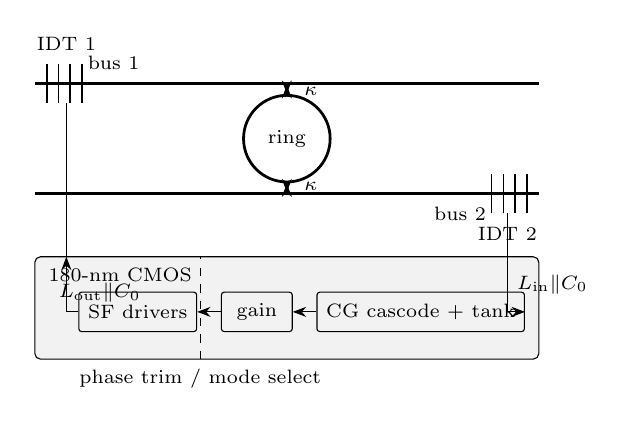
\begin{tikzpicture}[>=Stealth, font=\scriptsize, node distance=3mm]
% ring and buses
\draw[line width=1pt] (3.2,0.9) circle (0.55);
\draw[line width=1pt] (0.0,1.6) -- (6.4,1.6);
\draw[line width=1pt] (0.0,0.2) -- (6.4,0.2);
\node at (3.2,0.9) {ring};
\node[anchor=south] at (1.0,1.65) {bus 1};
\node[anchor=north] at (5.4,0.15) {bus 2};
\draw[<->] (3.2,1.47) -- (3.2,1.58); \node[anchor=west] at (3.3,1.5) {$\kappa$};
\draw[<->] (3.2,0.33) -- (3.2,0.22); \node[anchor=west] at (3.3,0.3) {$\kappa$};
% IDTs
\foreach \x in {0.15,0.3,0.45,0.6} \draw[line width=0.6pt] (\x,1.35) -- (\x,1.85);
\foreach \x in {5.8,5.95,6.1,6.25} \draw[line width=0.6pt] (\x,-0.05) -- (\x,0.45);
\node[anchor=south] at (0.4,1.9) {IDT 1};
\node[anchor=north] at (6.0,-0.1) {IDT 2};
% CMOS die
\draw[rounded corners=2pt, fill=gray!10] (0.0,-1.9) rectangle (6.4,-0.6);
\node[anchor=north west] at (0.05,-0.62) {180-nm CMOS};
\node[draw, rounded corners=1pt, minimum height=5mm, minimum width=1.3cm] (cg) at (4.9,-1.3) {CG cascode + tank};
\node[draw, rounded corners=1pt, minimum height=5mm, minimum width=0.9cm, left=of cg] (g2) {gain};
\node[draw, rounded corners=1pt, minimum height=5mm, minimum width=0.9cm, left=of g2] (sf) {SF drivers};
\draw[->] (cg) -- (g2); \draw[->] (g2) -- (sf);
\draw[->] (sf.west) -| (0.4,-0.6) node[midway, above, xshift=4mm] {\,$L_{\mathrm{out}}\|C_0$};
\draw[->] (6.0,-0.6) |- (cg.east) node[pos=0.25, right] {$L_{\mathrm{in}}\|C_0$};
\draw (0.4,1.35) -- (0.4,0.6) -- (0.4,-0.6);
\draw (6.0,-0.05) -- (6.0,-0.6);
\node[anchor=west] at (6.45,-1.3) {};
\draw[dashed] (2.1,-1.9) -- (2.1,-0.6); \node[anchor=north] at (2.1,-1.9) {phase trim / mode select};
\end{tikzpicture}
\caption{Transmission-mode oscillator: the SiN--LN ring with its two IDTs closes the loop through a CMOS sustaining amplifier whose port interfaces resonate the IDT static capacitance $C_0$.}
\label{fig:concept}
\end{figure}

\subsection{From ring physics to the extended mBVD circuit}
The ring is described by three round-trip quantities \cite{yariv2000}: the field attenuation $a$, the coupler through-transmission $t=\sqrt{1-\kappa^2}$ and the round-trip time $\tau_{\mathrm{rt}}=1/\mathrm{FSR}$. They follow from the measured quality factors as
\begin{equation}
1-a^2=\frac{\omega_0\tau_{\mathrm{rt}}}{Q_i},\qquad \kappa^2=\frac{\omega_0\tau_{\mathrm{rt}}}{Q_c},
\label{eq:rt}
\end{equation}
which give $a=\nart$, $t=\ntcp$ and $\kappa^2=\nkappatwo$\,\% for the device of \cite{ji2026}. The drop-port power transfer at resonance of an add--drop ring is
\begin{equation}
T_{\mathrm{drop}}=\frac{\kappa^4 a}{(1-t^2a)^2}\approx\frac{(1/Q_c)^2}{(1/Q_c+1/2Q_i)^2},
\label{eq:tdrop}
\end{equation}
where the approximation holds for small per-pass loss and shows that $T_{\mathrm{drop}}$ depends only on the ratio $Q_c/Q_i$, not on the (unknown) FSR. With the measured values, $T_{\mathrm{drop}}=-\nTdrop$~dB. This is the loss intrinsic to the under-coupled ring; the remaining $\nILidt$~dB of the measured 28.2~dB is split between the two ports and consists of IDT bidirectionality (3~dB per IDT), taper loss (below 1~dB per taper \cite{ji2026}), electrode resistance and the mismatch between the IDT impedance and 50~$\Omega$.

Each IDT is represented by its classical mBVD parasitics \cite{larson2000}: the static capacitance $C_0$ between the bus bars, a dielectric-loss resistance $R_0$ in parallel and an electrode resistance $R_s$ in series. The acoustic transfer between the two ports is a single series motional branch $L_m$--$C_m$--$R_m$ whose conductance at resonance is
\begin{equation}
G_m=\frac{1}{R_m}=G_{a0}\,\eta_t\sqrt{T_{\mathrm{drop}}},\quad L_m=\frac{Q_L R_m}{\omega_0},\quad C_m=\frac{1}{\omega_0^2 L_m},
\label{eq:mbvd}
\end{equation}
where $G_{a0}$ is the IDT radiation conductance at $f_0$ \cite{morgan2007} and $\eta_t$ the IDT-to-ring power efficiency (0.5 for a bidirectional IDT times a taper efficiency of 0.8). The product $G_{a0}\eta_t$ is calibrated once so that the two-port network, terminated in 50~$\Omega$, reproduces the measured $|S_{21}(f_0)|$; the result is $R_m=\nRm$~$\Omega$, $L_m=\nLmH$~mH, $C_m=\nCmaF$~aF with $C_0=\nCzeropF$~pF, $R_0=\nRzerok$~k$\Omega$ and $R_s=\nRs$~$\Omega$ (Table~\ref{tab:res}). The effective coupling $k_{\mathrm{eff}}^2=C_m/C_0=\nkeff\times10^{-6}$ is four orders of magnitude below that of an FBAR; this single number drives the topology choice of Section~\ref{sec:codesign}. Spurious transverse modes are added as parallel LCR branches with a relative coupling $k_s$ and a lower $Q_s$. The IDT transduction envelope $|H_{\mathrm{IDT}}|^2=\mathrm{sinc}^2\!\big[N(f-f_0)/f_0\big]$ for $N$ finger pairs \cite{morgan2007} multiplies the transfer admittance; it is the only broadband frequency selectivity in the loop and is used in Section~\ref{sec:mode}.

\begin{table}[!t]
\caption{Resonator parameters: measured \cite{ji2026}, assumed and derived}
\label{tab:res}
\centering
\begin{tabular}{llr}
\toprule
Quantity & Origin & Value \\
\midrule
$f_0$ & measured & $\nfzeroMHz$ MHz\\
$Q_L$, $Q_i$, $Q_c$ & measured & $\nQL$, $\nQi$, $\nQc$\\
$|S_{21}(f_0)|$, 50 $\Omega$ & measured & $-28.2$ dB\\
$v_g$, $m$, $R$ & assumed / derived & 3600 m/s, 175, $\nradiusum$ $\mu$m\\
FSR, $\tau_{\mathrm{rt}}$ & derived & $\nFSRMHz$ MHz, $\ntaurtns$ ns\\
$a$, $t$, $\kappa^2$ & derived (\ref{eq:rt}) & $\nart$, $\ntcp$, $\nkappatwo$\,\%\\
$T_{\mathrm{drop}}$ & derived (\ref{eq:tdrop}) & $-\nTdrop$ dB\\
$C_0$, $R_0$, $R_s$ & assumed (IDT) & $\nCzeropF$ pF, $\nRzerok$ k$\Omega$, $\nRs$ $\Omega$\\
$G_{a0}\eta_t$ & calibrated to $S_{21}$ & $\nGazeromS\times0.4$ mS\\
$R_m$, $L_m$, $C_m$ & derived (\ref{eq:mbvd}) & $\nRm$ $\Omega$, $\nLmH$ mH, $\nCmaF$ aF\\
$k_{\mathrm{eff}}^2=C_m/C_0$ & derived & $\nkeff\times10^{-6}$\\
TCF & assumed (LN) & $-70$ ppm/K\\
\bottomrule
\end{tabular}
\end{table}

\subsection{The delay element}
A single LCR branch is a Lorentzian: it has the right loaded linewidth and phase slope at $f_0$ but no memory of the ring circumference, so it predicts a single resonance where the device has a comb, and it cannot represent the half-round-trip propagation phase that the signal acquires between the two couplers. The model therefore implements the ring as a recirculating delay loop,
\begin{equation}
x(t)=\kappa\,v_1(t-\tfrac{\tau_{\mathrm{rt}}}{2})+t\,a\,x(t-\tau_{\mathrm{rt}}),\qquad
i_2(t)=G_m'\,\kappa\sqrt{a}\,x(t-\tfrac{\tau_{\mathrm{rt}}}{2}),
\label{eq:delay}
\end{equation}
where $x$ is the circulating field, $v_1$ the voltage at port~1, $i_2$ the short-circuit current injected into port~2 and $G_m'=G_m/\sqrt{T_{\mathrm{drop}}}$ a scale factor that makes the transfer at $f_0$ identical to the mBVD branch. In the frequency domain (\ref{eq:delay}) is $\kappa^2\sqrt a\,e^{-j\omega\tau_{\mathrm{rt}}/2}/(1-t^2a\,e^{-j\omega\tau_{\mathrm{rt}}})$: a comb of Lorentzians of width $f_0/Q_L$ spaced by the FSR, each carrying the propagation phase $-\omega\tau_{\mathrm{rt}}/2$. Two consequences follow that the BVD branch misses. (i) Adjacent comb modes differ in loop phase by $\pi\,\mathrm{FSR}\,\tau_{\mathrm{rt}}=\pi$: of two neighbouring modes, only one can satisfy the Barkhausen phase condition for a given amplifier phase, and the nearest in-phase competitors are at $f_0\pm2\,\mathrm{FSR}$. (ii) The group delay of the ring, $\tau_g=2Q_L/\omega_0=\ntaurtns\cdot 0+5.7$~$\mu$s at resonance, sets the start-up time constant together with the loop gain. Fig.~\ref{fig:resonator}(a) compares the comb and the single-branch responses in a 50-$\Omega$ system; Fig.~\ref{fig:resonator}(b) shows the design mode.

\begin{figure}[!t]
\centering
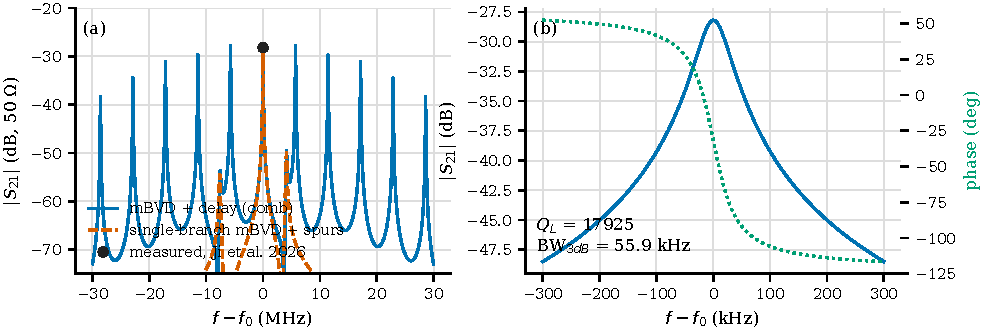
\includegraphics[width=\linewidth]{fig_resonator}
\caption{(a) $|S_{21}|$ of the calibrated model in a 50-$\Omega$ system: the delay-element comb (solid) and the single-branch mBVD with two spurious branches (dashed); the dot is the measured value of \cite{ji2026}. (b) Magnitude and phase of the design mode.}
\label{fig:resonator}
\end{figure}

\subsection{Verilog-A implementation}
The model is written as a true floating four-terminal element: the motional chain is driven by $v_1-v_2$ through an internal node and its current is copied into both ports with their own return terminals, which gives $Y_{11}=Y_{22}=Y_m$, $Y_{12}=Y_{21}=-Y_m$ without a common-ground assumption, so that the IDT bus bars can be driven differentially. A parameter selects the single-branch form (\texttt{mode=0}, used for PSS/Pnoise because shooting methods converge faster without long delays) or the delay-loop form (\texttt{mode=1}, implemented with \texttt{absdelay}, used for mode selection and start-up). Thermal noise is attached to every resistive element, an optional $1/f$ term on $R_m$ represents resonator flicker, the temperature coefficient of frequency acts on $f_0$ and FSR, and an optional thermal node models self-heating from the power dissipated in $R_m$. The cell therefore behaves as a noise source in Pnoise, which a behavioural S-parameter block would not.

\section{Sustaining-Amplifier Co-Design}\label{sec:codesign}

\subsection{Why the Pierce topology fails}
In a Pierce oscillator the resonator must look inductive, which happens only between the series and parallel resonances, $f_p-f_s=f_s\,C_m/(2C_0)$. For the two-port ring with $C_m/C_0=\nkeff\times10^{-6}$ this window is $\nwindow$~Hz wide at 1~GHz: an amplifier phase error of a fraction of a degree pushes the loop out of it. In addition the critical transconductance with the IDT capacitances acting as $C_1=C_2=C_0$ is $g_{m,\mathrm{crit}}=\omega_0^2C_0^2R_m=\ngmcrit$~mS \cite{vittoz1988}, i.e. $\ngmthreex$~mS (about $\nPthreex$~mW in 180-nm CMOS) for the customary $3\times$ margin, with no mode-selection control. The same argument excludes Colpitts and cross-coupled negative-resistance cores. The ring must be used as what it is, a transmission element in series resonance: the loop closes through it, the amplifier is a transimpedance block and the oscillation condition is $|Z_T|>R_m+R_{\mathrm{ext}}$ at zero loop phase, where $R_{\mathrm{ext}}$ is the sum of the real port impedances of the amplifier.

\subsection{Loss recovery by port-impedance co-design}
Fig.~\ref{fig:il} shows the transducer gain of the calibrated resonator at $f_0$ between two equal real terminations $R$. Without inductors the optimum is near 200~$\Omega$ and only 5~dB better than the 50-$\Omega$ value, because the motional current is shunted by the 187-$\Omega$ reactance of $C_0$. When a shunt inductor of $Q_L$ resonates $C_0$ at each port, the gain approaches the drop-port limit for $R\approx1$--2~k$\Omega$: with on-chip inductors of $Q_L=8$ the best gain is $-\nILbestQeight$~dB, a recovery of $\nILrecQeight$~dB, and with $Q_L=30$ (bond-wire or 0402 inductors) $-\nILbestQthreezero$~dB. In the transmission-mode loop the relevant figure is not a transducer gain but the ratio of the port-2 short-circuit current to the port-1 drive voltage relative to $1/R_m$; for the amplifier of Section~\ref{sec:amp} this \emph{loop loss} is $\nloopLoss$~dB ($\nloopLossNoL$~dB without inductors), i.e. essentially the full motional current is available to the amplifier.

\begin{figure}[!t]
\centering
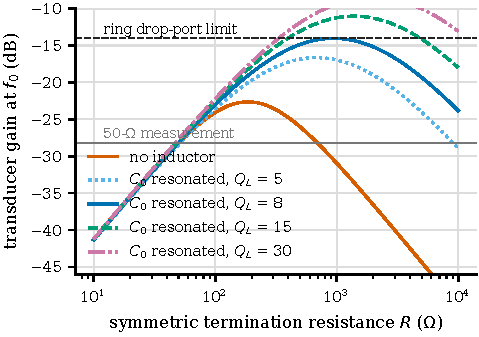
\includegraphics[width=\linewidth]{fig_il_recovery}
\caption{Transducer gain of the resonator at $f_0$ versus symmetric termination resistance, with and without $C_0$-resonating shunt inductors of different $Q_L$. The 50-$\Omega$ measurement and the ring drop-port limit (\ref{eq:tdrop}) are marked.}
\label{fig:il}
\end{figure}

\subsection{Transmission-mode differential sustaining amplifier}\label{sec:amp}
Fig.~\ref{fig:amp} shows the circuit (180-nm bulk CMOS, 1.8~V). Both IDTs are floating and driven differentially. The input is a common-gate (CG) differential pair M1 with cascode devices M1c and a differential LC tank ($L_t=\nLt$~nH, $Q_t=8$, $R_p=\nRptank$~$\Omega$) as the load; the low input impedance $2/g_{m1}=\nRext\cdot0+53$~$\Omega$ keeps the electrical loading of the motional branch small ($R_{\mathrm{ext}}=\nRext$~$\Omega$, $Q_e=\nQe$) and senses the motional current directly. The port-2 inductor $L_{\mathrm{in}}=\nLin$~nH that resonates $C_0$ is centre-tapped and the tap carries the bias current of the CG pair: the noise of the tail current source then appears as a common-mode signal and is rejected, which removed the dominant noise term of the first design iteration (a grounded-tail CG stage had $F=12.8$~dB in transistor-level simulation; the centre-tapped version has $\nngF$~dB). The cascode isolates the tank from the output conductance of M1. Two resistor-loaded differential pairs (M2 with a PMOS current-source assist that carries $\nItwop$~mA of the $\nItwo$~mA bias so that $R_{L2}=\nRLtwo$~$\Omega$ fits the 1.8-V headroom, and M3 with $R_{L3}=\nRLthree$~$\Omega$) provide the remaining gain and the amplitude limiting; source followers M4 drive IDT~1 through the second resonating inductor $L_{\mathrm{out}}$, which removes the reactive current of $C_0$ from the driver. The current budget is $2\times(\nIone+\nItwo+\nIthree+\nIfour)=\nIdc$~mA, i.e. $\nPdc$~mW.

\begin{figure*}[!t]
\centering
\begin{circuitikz}[scale=0.78, transform shape, font=\footnotesize]
% port 2 inductor, centre tapped
\draw (0,0) node[left]{$p_2$} to[L, l_=$L_{\rm in}/2$] (0,-2) node (ct) {} to[L, l_=$L_{\rm in}/2$] (0,-4) node[left]{$n_2$};
\draw (0,-2) -- (1,-2) node[nmos, anchor=D, rotate=0] (mt1) {};
\node at (1.9,-2.6) {M$_{t1}$};
\draw (mt1.S) -- ++(0,-0.5) node[ground]{};
\draw (mt1.G) -- ++(-0.6,0) node[left]{$V_{bn}$};
\draw (0,-2) to[C, l=$C_{ct}$] (0,-2) ;
% CG pair
\draw (0,0) -- (2.5,0) node[nmos, anchor=S, rotate=90] (m1a) {};
\draw (0,-4) -- (2.5,-4) node[nmos, anchor=S, rotate=90] (m1b) {};
\node at (3.0,0.6) {M$_{1a}$}; \node at (3.0,-3.4) {M$_{1b}$};
\draw (m1a.G) -- ++(0,0.8) node[above]{$V_{b1}$};
\draw (m1b.G) -- ++(0,0.8) node[above]{$V_{b1}$};
% cascode
\draw (m1a.D) -- ++(0.6,0) node[nmos, anchor=S, rotate=90] (m1ca) {};
\draw (m1b.D) -- ++(0.6,0) node[nmos, anchor=S, rotate=90] (m1cb) {};
\draw (m1ca.G) -- ++(0,0.8) node[above]{$V_{bc}$};
\draw (m1cb.G) -- ++(0,0.8) node[above]{$V_{bc}$};
% tank
\draw (m1ca.D) -- ++(1.2,0) coordinate (d1a);
\draw (m1cb.D) -- ++(1.2,0) coordinate (d1b);
\draw (d1a) to[L, l=$L_t/2$] ++(0,-1.6) coordinate (vddt) to[L, l=$L_t/2$] (d1b);
\draw (vddt) -- ++(0.9,0) node[right]{$V_{DD}$};
\draw ($(d1a)+(-0.5,0)$) to[vC, l=$C_t$ (trim)] ($(d1b)+(-0.5,0)$);
% gain stages as blocks
\draw (d1a) -- ++(1.6,0) coordinate (s2in);
\draw (d1b) -- ++(1.6,0) coordinate (s2inb);
\draw[rounded corners] ($(s2in)+(0,0.5)$) rectangle ($(s2inb)+(2.4,-0.5)$);
\node at ($(s2in)+(1.2,-2)$) {\shortstack{M$_2$, PMOS assist\\$R_{L2}$ \nRLtwo\,$\Omega$}};
\draw ($(s2in)+(2.4,0)$) -- ++(0.8,0) coordinate (s3in);
\draw ($(s2inb)+(2.4,0)$) -- ++(0.8,0) coordinate (s3inb);
\draw[rounded corners] ($(s3in)+(0,0.5)$) rectangle ($(s3inb)+(2.0,-0.5)$);
\node at ($(s3in)+(1.0,-2)$) {\shortstack{M$_3$\\$R_{L3}$ \nRLthree\,$\Omega$}};
\draw ($(s3in)+(2.0,0)$) -- ++(0.8,0) coordinate (s4in);
\draw ($(s3inb)+(2.0,0)$) -- ++(0.8,0) coordinate (s4inb);
\draw[rounded corners] ($(s4in)+(0,0.5)$) rectangle ($(s4inb)+(1.6,-0.5)$);
\node at ($(s4in)+(0.8,-2)$) {\shortstack{M$_4$\\SF drivers}};
% output port with Lout
\draw ($(s4in)+(1.6,0)$) to[C, l=$C_c$] ++(1.4,0) coordinate (p1) node[right]{$p_1$};
\draw ($(s4inb)+(1.6,0)$) to[C, l=$C_c$] ++(1.4,0) coordinate (n1) node[right]{$n_1$};
\draw ($(p1)+(0.9,0)$) to[L, l=$L_{\rm out}$] ($(n1)+(0.9,0)$);
\end{circuitikz}
\caption{Transmission-mode sustaining amplifier (one of the two symmetric halves of each stage is drawn for the CG cascode). The motional current from IDT~2 enters the common-gate pair through the centre-tapped $C_0$-resonating inductor $L_{\rm in}$; the stage-1 tank with its trim varactor $C_t$ sets the loop phase; the driver output resonates $C_0$ of IDT~1 with $L_{\rm out}$.}
\label{fig:amp}
\end{figure*}

A behavioural model of the chain, $Z_T(f)=k_{\mathrm{impl}}\,Z_{\mathrm{tank}}(f)A_2A_3A_4$ with first-order poles at each node, is used for design exploration; its gain is calibrated to the transistor-level simulation through the single factor $k_{\mathrm{impl}}=\nkimpl$~dB, which collects the loading of the tank by the cascode and stage-2 capacitances, the finite PMOS output resistance and the source-follower loss. The noise and resonator parts of the behavioural model need no calibration: the circuit-derived loop noise factor of Section~\ref{sec:noise} ($\nFmodel$~dB) agrees with the transistor-level value ($\nngF$~dB) within 0.3~dB.

\subsection{Phase trim and mode selection}\label{sec:mode}
The loop phase at $f_0$ is zeroed with a varactor on the stage-1 tank (a detuning $\delta$ shifts the phase by $-\arctan(2Q_t\delta)$, so $\pm10$\,\% of $C_t$ gives $\pm58^\circ$) and by the choice of the loop polarity, which costs nothing in a differential amplifier. The nominal design needs $\ntrim^\circ$ of trim; over the Monte Carlo population of Section~\ref{sec:mc} the requirement spans $\nmcTrimMin^\circ$ to $\nmcTrimMax^\circ$, inside the varactor range. Fig.~\ref{fig:loop}(b) shows the loop gain across the comb computed with the delay-element model: the odd-order neighbours ($k=\pm1,\pm3,\dots$) have $180^\circ$ loop phase and cannot oscillate, so the nearest in-phase competitor is at $k=\nmodeCompK$ ($\nmodeCompMHz$~MHz from $f_0$) with a margin of only $\nmodeMargin$~dB against the IDT envelope of the baseline $N=\nNidt$ finger pairs. This small margin explains the mode hopping used for tuning in \cite{ji2026}. Fig.~\ref{fig:modemargin} shows the margin versus $N$: the first null of $\mathrm{sinc}^2[N(f-f_0)/f_0]$ falls on $f_0\pm2\,\mathrm{FSR}$ when
\begin{equation}
N=\frac{f_0}{2\,\mathrm{FSR}}=\nNopt,
\label{eq:nopt}
\end{equation}
where the margin reaches $\nmarginNopt$~dB without any extra filter. Rule (\ref{eq:nopt}) couples the transducer design to the ring circumference and is, to the author's knowledge, new; it increases $C_0$ proportionally to $N$, which the port inductors absorb, and the IDT bandwidth then equals $2\,\mathrm{FSR}$, which still leaves the phase-trim tuning within one mode. Conversely, if mode hopping is wanted as a coarse tuning mechanism, $N$ is kept small and the trim word selects $k$.

\begin{figure}[!t]
\centering
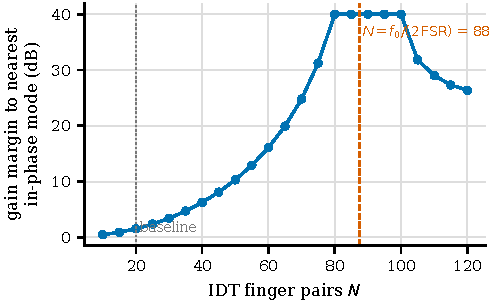
\includegraphics[width=\linewidth]{fig_mode_margin}
\caption{Loop-gain margin of the design mode against the nearest in-phase comb mode versus the number of IDT finger pairs $N$; the optimum (\ref{eq:nopt}) places the IDT nulls on $f_0\pm2\,\mathrm{FSR}$.}
\label{fig:modemargin}
\end{figure}

\subsection{Noise analysis}\label{sec:noise}
All noise sources are referred to the port-2 node as Norton currents and compared with the thermal noise of $R_m$, which is the only unavoidable source. With $Y_{\mathrm{src}}$ the total admittance seen by the CG pair and $g_{md}=g_{m1}/2$ its differential transconductance, the CG channel noise referred to the input is $4kT\gamma|Y_{\mathrm{src}}|^2/g_{md}$, which is why $L_{\mathrm{in}}$ matters: without it $|Y_{\mathrm{src}}|$ is dominated by $\omega C_0$ and the CG term alone is $+6.7$~dB. The tank loss contributes $4kT/R_p$ and the stage-2 input noise $v_{n2}^2/R_p^2$, both divided by the fraction of the port current that enters the CG devices. The resulting budget (Table~\ref{tab:noise}) gives $F=\nFmodel$~dB, dominated by the CG term ($\nFpartCG$~dB), the input inductor loss ($\nFpartLin$~dB) and the tank loss ($\nFparttank$~dB); inductor $Q$ is therefore the first lever on the noise floor (Section~\ref{sec:pn}). The transistor-level simulation (Section~\ref{sec:results}) returns $\nngF$~dB with the same ranking of contributors.

\begin{table}[!t]
\caption{Loop noise budget referred to the thermal noise of $R_m$ (behavioural model, nominal design)}
\label{tab:noise}
\centering
\begin{tabular}{lr}
\toprule
Source & relative (dB) \\
\midrule
$R_m$ (reference) & 0.0\\
other resonator resistances ($R_s$, $R_0$, driver $R_{\rm out}$) & $\nFpartresother$\\
$L_{\rm in}$ loss ($Q_L=\nQLind$) & $\nFpartLin$\\
CG pair channel noise & $\nFpartCG$\\
stage-1 tank loss & $\nFparttank$\\
stage-2 input-referred & $\nFpartstagetwo$\\
driver excess noise & $\nFpartdriver$\\
\midrule
total $F$ & $\nFmodel$\\
transistor-level (ngspice, per-generator) & $\nngF$\\
\bottomrule
\end{tabular}
\end{table}

\section{Simulation Results}\label{sec:results}
The pre-layout results are obtained with the behavioural model calibrated as described above and with transistor-level ngspice simulation of the complete loop using generic 180-nm BSIM3v3 model cards; the Spectre/foundry-PDK run of Section~\ref{sec:flow} replaces them for the post-layout version.

\subsection{Open loop, start-up and steady state}
Fig.~\ref{fig:loop}(a) shows the open-loop gain with the loop broken at port~1 and terminated by replicas of the driver and port impedances. The transistor-level loop gain at $f_0$ is $\nngTzero$~dB with the loop phase trimmed to $\nngPhase^\circ$ by the tank capacitance ($C_t=\nngCt$~fF); the behavioural model reproduces the shape of the response once calibrated. The linear start-up time constant is $\tau=2Q_e/[\omega_0(|T|-1)]=\ntauStart$~$\mu$s, and the transient simulation of Fig.~\ref{fig:startup}(a) reaches 90\,\% of the final envelope at $\nngTstart$~$\mu$s. In steady state (Fig.~\ref{fig:startup}(b)) the oscillator runs at $\nngFosc$~MHz ($\nngDf$~kHz from the resonator centre, within the trim resolution), the differential swing at IDT~1 is $\nngVpone$~V, the motional current is $\nngIm$~mA peak and the power dissipated in $R_m$, i.e. the acoustic power delivered to the ring, is $\nngPrm$~dBm. The second and third harmonics at the resonator port are $\nngHDtwo$ and $\nngHDthree$~dBc: the ring itself filters the limiting-stage distortion.

\begin{figure*}[!t]
\centering
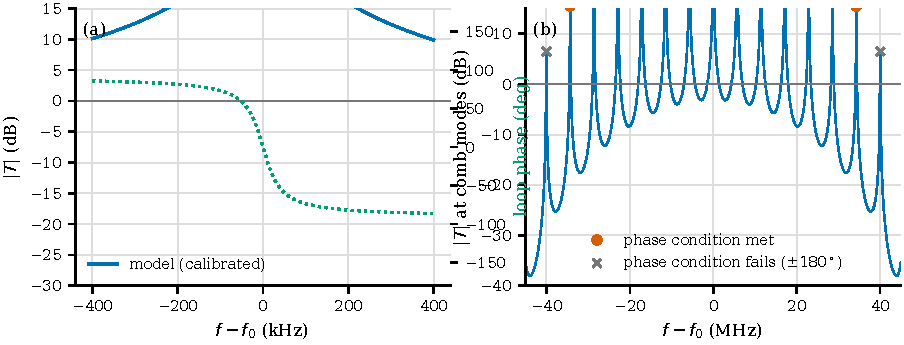
\includegraphics[width=\textwidth]{fig_loopgain}
\caption{(a) Open-loop gain and phase around $f_0$: behavioural model (calibrated) and transistor-level ngspice. (b) Loop gain across the comb from the delay-element model, marking the modes that satisfy and fail the phase condition.}
\label{fig:loop}
\end{figure*}

\begin{figure*}[!t]
\centering
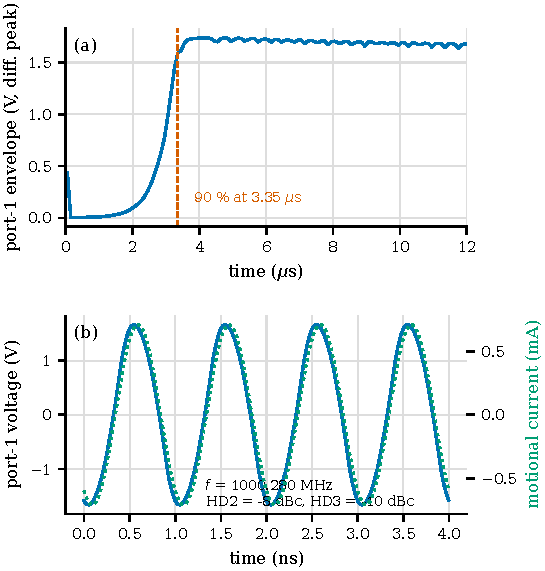
\includegraphics[width=\textwidth]{fig_startup}
\caption{Transistor-level transient: (a) envelope of the differential voltage at IDT~1 from a 50-$\mu$A, 1-ns kick; (b) steady-state waveform and motional current.}
\label{fig:startup}
\end{figure*}

\subsection{Phase noise}\label{sec:pn}
With $F$, $Q_e$ and the ring power $P_s$ taken from the circuit, the Leeson--Cutler form \cite{leeson1966,razavi2012}
\begin{equation}
\mathcal{L}(\Delta f)=\frac{FkT}{2P_s}\Big[1+\Big(\frac{f_0}{2Q_e\Delta f}\Big)^2\Big]\Big(1+\frac{f_c}{\Delta f}\Big)
\label{eq:leeson}
\end{equation}
has a single free parameter, the effective flicker corner $f_c$ after up-conversion, which depends on the waveform symmetry and on the PDK flicker model \cite{hajimiri1998}; it is swept over 10, 30 and 100~kHz and the Spectre Pnoise run resolves it. The floor is $\nPNfloor$~\dBc, the half-bandwidth $f_0/2Q_e=\nhalfBW$~kHz, and the resulting curves are shown in Fig.~\ref{fig:pn} with the literature references of Table~\ref{tab:cmp}. For $f_c=30$~kHz the oscillator reaches $\nPNonek$, $\nPNonezerok$, $\nPNonezerozerok$ and $\nPNoneM$~\dBc\ at 1~kHz, 10~kHz, 100~kHz and 1~MHz. Fig.~\ref{fig:pnterms} separates the floor, the $Q_e$-limited $1/f^2$ region and the flicker $1/f^3$ region: the close-in noise is set by $Q_e$ and $f_c$, the far-out noise by $F/P_s$. Fig.~\ref{fig:pnsens} quantifies the two design levers: raising the inductor $Q$ from 8 to 30 improves $F$ to $\nFQthreezero$~dB and $\mathcal{L}(100\,\mathrm{kHz})$ to $\nPNonezerozerokQthreezero$~\dBc, and every 3~dB of additional ring drive power lowers the whole curve by 3~dB until the resonator nonlinearity, not characterised in \cite{ji2026}, sets in. The figure of merit $\mathrm{FoM}=-\mathcal{L}+20\log(f_0/\Delta f)-10\log(P_{dc}/\mathrm{mW})$ is $\nFoMonezerozerok$~dB at 100~kHz.

\begin{figure}[!t]
\centering
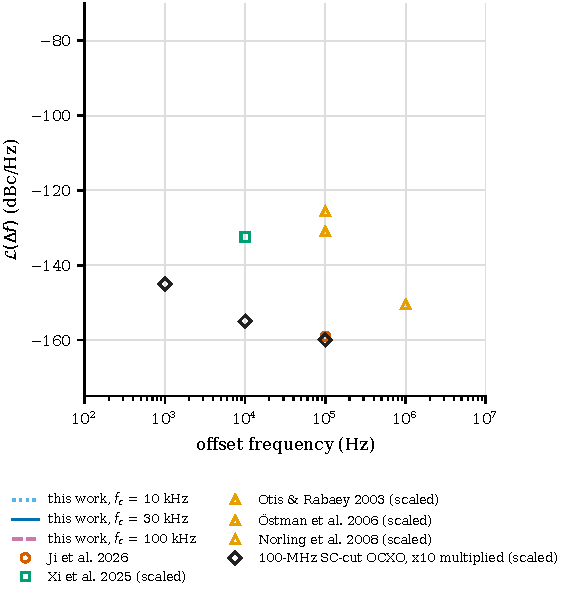
\includegraphics[width=\linewidth]{fig_phase_noise}
\caption{Predicted phase noise (\ref{eq:leeson}) with circuit-derived $F$, $Q_e$ and $P_s$ for three flicker corners, compared with published SiN--LN, SAW, FBAR and quartz references (values scaled to 1~GHz by $20\log(f_0/f_{\rm ref})$ where marked).}
\label{fig:pn}
\end{figure}

\begin{figure}[!t]
\centering
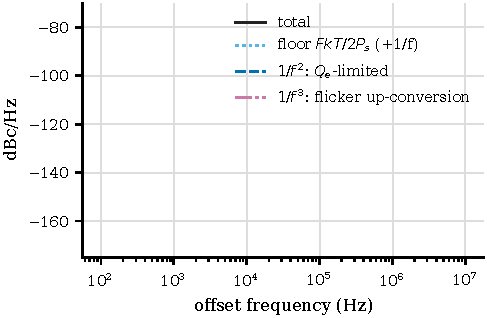
\includegraphics[width=\linewidth]{fig_pn_terms}
\caption{Decomposition of the phase noise into the thermal floor, the $Q_e$-limited $1/f^2$ term and the flicker $1/f^3$ term ($f_c=30$~kHz).}
\label{fig:pnterms}
\end{figure}

\begin{figure*}[!t]
\centering
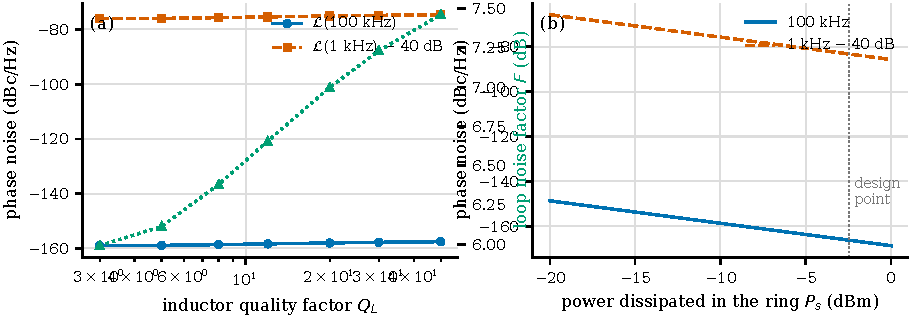
\includegraphics[width=\textwidth]{fig_pn_sensitivity}
\caption{(a) Phase noise and loop noise factor versus the quality factor of the three on-chip inductors. (b) Phase noise versus the power dissipated in the ring.}
\label{fig:pnsens}
\end{figure*}

\subsection{Process, resonator and temperature variations}\label{sec:mc}
Fig.~\ref{fig:mc} shows 300 Monte Carlo trials over $Q_i$ (log-normal, 20\,\%), $Q_c$ (30\,\%), $f_0$ (500~ppm), $C_0$ (10\,\%), IDT conductance (15\,\%), transistor $g_m$ and bias (10\,\%), inductance (8\,\%), inductor $Q$ (15\,\%) and supply (3\,\%), with the phase trim re-calibrated for each trial as the on-chip calibration would do. The loop gain is $\nmcTzeromean\pm\nmcTzerostd$~dB (minimum $\nmcTzeromin$~dB) and the start-up yield is $\nmcYield$\,\%; $\mathcal{L}(100\,\mathrm{kHz})$ is $\nmcPNonezerozeromean\pm\nmcPNonezerozerostd$~\dBc\ and $\mathcal{L}(1\,\mathrm{kHz})$ $\nmcPNonemean\pm\nmcPNonestd$~\dBc, the spread coming almost entirely from $Q_c$ through $Q_e$ ($\nmcQeMean\pm\nmcQeStd$). Over $-40$ to $85^\circ$C (Fig.~\ref{fig:temp}) the frequency follows the assumed LN TCF ($\ntempDfRange$~ppm span), the loop gain stays between $\ntempTzeromin$ and $\ntempTzeromax$~dB and $\mathcal{L}(100\,\mathrm{kHz})$ between $\ntempPNmin$ and $\ntempPNmax$~\dBc. A programmable stage-2 bias (two bits) is included in the layout to recover the low-gain tail of the distribution.

\begin{figure*}[!t]
\centering
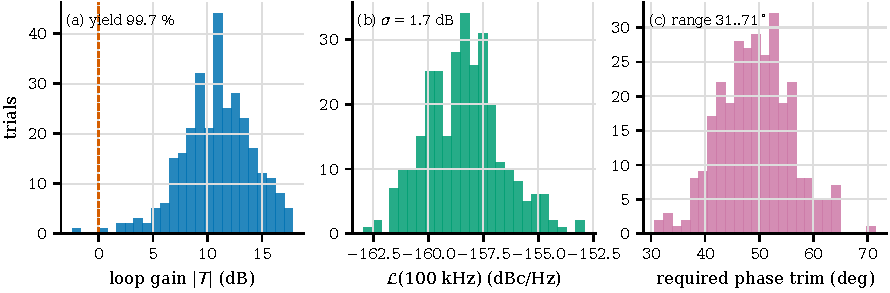
\includegraphics[width=\textwidth]{fig_montecarlo}
\caption{Monte Carlo (300 trials): (a) loop gain, (b) $\mathcal{L}(100\,\mathrm{kHz})$, (c) required phase trim.}
\label{fig:mc}
\end{figure*}

\begin{figure*}[!t]
\centering
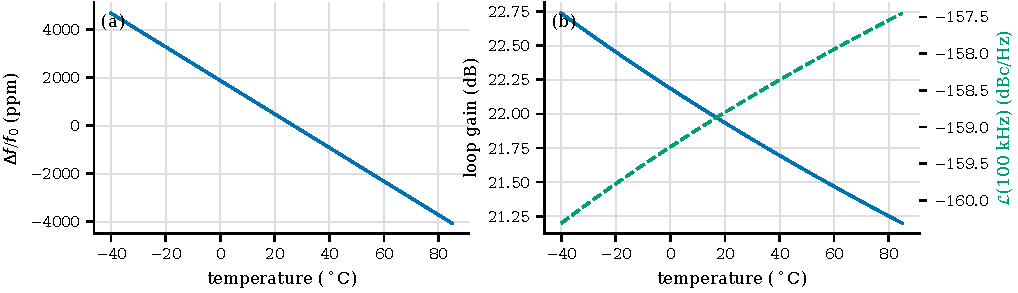
\includegraphics[width=\textwidth]{fig_temperature}
\caption{Temperature behaviour: (a) frequency drift with the LN TCF, (b) loop gain and phase noise at 100~kHz.}
\label{fig:temp}
\end{figure*}

\subsection{Short-term stability}
The Allan deviation obtained from (\ref{eq:leeson}) with the IEEE~1139 transfer function \cite{ieee1139,rubiola2009} (Fig.~\ref{fig:adev}) is $\nadevonezerous$ at 10~$\mu$s, $\nadevonems$ at 1~ms and $\nadevones$ at 1~s, the flicker floor being set by $f_c$; it excludes temperature and ageing drift.

\begin{figure}[!t]
\centering
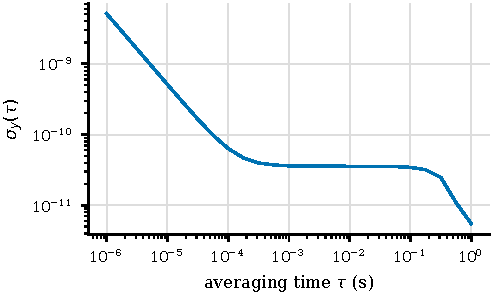
\includegraphics[width=\linewidth]{fig_adev}
\caption{Allan deviation computed from the predicted phase-noise spectrum.}
\label{fig:adev}
\end{figure}

\subsection{Comparison}
Table~\ref{tab:cmp} compares the predicted performance with the bench-instrument oscillator on the same resonator \cite{ji2026}, a 1-GHz SAW oscillator with a phononic-band-gap edge mode \cite{xi2025}, FBAR oscillators in CMOS and SiGe \cite{otis2003,ostman2006,norling2008} and a state-of-the-art 100-MHz SC-cut quartz OCXO multiplied to 1~GHz \cite{rubiola2009}. At 100~kHz the integrated design is within 1~dB of the bench oscillator while dissipating $\nPdc$~mW instead of the watts of an instrument chain, and it is more than 25~dB better than the FBAR--CMOS references; at 1~kHz it sits between FBAR and multiplied quartz, limited by the flicker corner of the 180-nm devices, which a thicker-oxide input pair or a chopped bias can reduce.

\begin{table*}[!t]
\caption{Comparison with published acoustic-resonator oscillators near 1--2 GHz (phase noise in \dBc; $\ast$ scaled to 1~GHz)}
\label{tab:cmp}
\centering
\begin{tabular}{llccccccc}
\toprule
Work & Resonator / technology & $f_0$ (MHz) & 1 kHz & 10 kHz & 100 kHz & 1 MHz & $P_{dc}$ (mW) & FoM$_{100\,\rm kHz}$ (dB)\\
\midrule
This work (pre-layout, $f_c$ = 30 kHz) & SiN--LN ring + 180-nm CMOS & $\nfzeroMHz$ & $\nPNonek$ & $\nPNonezerok$ & $\nPNonezerozerok$ & $\nPNoneM$ & $\nPdc$ & $\nFoMonezerozerok$\\
This work (post-layout, Spectre) & SiN--LN ring + 180-nm CMOS & \tbd & \tbd & \tbd & \tbd & \tbd & \tbd & \tbd\\
Ji \textit{et al.} 2026 \cite{ji2026} & SiN--LN ring, bench amplifier & 1001.15 & -- & -- & $-159.0$ & -- & -- & --\\
Xi \textit{et al.} 2025 \cite{xi2025} & LN SAW, band-gap edge mode & 1000 & -- & $-132.5$ & -- & -- & -- & --\\
Otis and Rabaey 2003 \cite{otis2003} & AlN FBAR, 0.13-$\mu$m CMOS Pierce & 1900 & -- & -- & $-120$ & -- & 0.3 & 211\\
\"Ostman \textit{et al.} 2006 \cite{ostman2006} & above-IC AlN FBAR, SiGe & 2100 & -- & -- & -- & $-144.1$ & -- & --\\
Norling \textit{et al.} 2008 \cite{norling2008} & monolithic AlN TFBAR, SiGe & 2000 & -- & -- & $-125$ & -- & -- & --\\
100-MHz SC-cut OCXO $\times10^\ast$ \cite{rubiola2009} & quartz, multiplied & 1000 & $-145$ & $-155$ & $-160$ & -- & $>$1000 & --\\
\bottomrule
\end{tabular}
\end{table*}

\section{Cadence Implementation Flow}\label{sec:flow}
The Verilog-A cell, the Spectre netlists of the amplifier and of the two testbenches, and the OCEAN scripts are released with the manuscript. The open-loop testbench breaks the loop with an \texttt{iprobe} at the CG input, the lowest-impedance node, and runs \texttt{stb} over $\pm60$~MHz to reproduce Fig.~\ref{fig:loop}; the oscillator testbench runs a 60-$\mu$s transient, a shooting PSS with \texttt{tstab} equal to the transient length (the loaded $Q$ makes a cold PSS start fail) and a Pnoise sweep from 100~Hz to 10~MHz with \texttt{noisetype=pm} at the IDT~1 port. Corner (tt/ss/ff/sf/fs, $-40/27/85^\circ$C, $\pm10$\,\% supply) and Monte Carlo scripts mirror Section~\ref{sec:mc}. The layout plan places the three inductors with 50-$\mu$m keep-outs, common-centroid differential pairs, 70-$\mu$m IDT pads with 60-fF ESD devices and a two-bit stage-2 bias trim in a $0.55\times0.45$~mm$^2$ core; Calibre DRC, LVS (the resonator as an LVS box bound to four pads) and xRC extraction run from the provided scripts, after which the PSS/Pnoise testbench is re-run on the extracted view and the post-layout column of Table~\ref{tab:cmp} is filled by the same data pipeline. The transistor-level pre-layout numbers of Section~\ref{sec:results} were obtained with generic BSIM3v3 model cards; the foundry PDK (SCL, TSMC or UMC 180~nm) is substituted through a single wrapper file, so the flow is PDK-agnostic.

\section{Conclusion}
A phononic ring resonator on SiN--LN is a two-port transmission element with a comb of modes and a vanishing effective coupling, and it has to be treated as such. The extended mBVD--delay model proposed here is derived from four measured quantities, carries the propagation phase and the mode comb, runs in Spectre PSS/Pnoise as a noise-generating Verilog-A cell, and makes the three decisive design facts quantitative: half of the measured 28-dB loss is recoverable on chip, the Pierce family is excluded, and the mode-selection margin is set by the IDT pair count through $N\approx f_0/2\,\mathrm{FSR}$. The transmission-mode CMOS sustaining amplifier with centre-tapped $C_0$-resonating port inductors reaches a loop noise factor near 6.7~dB and a predicted $\nPNonezerozerok$~\dBc\ at 100~kHz for $\nPdc$~mW, within 1~dB of the bench demonstration on the same resonator and 25~dB beyond FBAR--CMOS oscillators, with a $\nmcYield$\,\% start-up yield over process and resonator variations. The released Cadence flow carries the design to layout, DRC/LVS, extraction and post-layout phase-noise verification; measured results on a bonded SiN--LN/CMOS assembly are the next step.

\section*{Acknowledgment}
The author thanks the Department of ECE, Velalar College of Engineering and Technology, for computing resources, and acknowledges the open-source ngspice and TeX communities.

\bibliographystyle{IEEEtran}
\bibliography{refs}

\begin{IEEEbiographynophoto}{M. Nisha Angeline}
is Professor and Head of the Department of Electronics and Communication Engineering, Velalar College of Engineering and Technology, Thindal, Erode, India. Her research interests include plasma technology, quantum computing, biomedical device design, VLSI and advanced chip technology, antenna design and open-source EDA.
\end{IEEEbiographynophoto}

\end{document}
